\apendice{Especificación de diseño}

\section{Introducción}
En este anexo se expone el diseño que se ha usado para llevar a cavo los objetivos anteriores. Como se manejan los datos, la arquitectura y modelos.

\section{Diseño de datos}
La aplicación cuenta con el modelado de los siguientes:

\begin{itemize}
\item \textbf{Usuario:} la entidad del usuario es una entidad simple la cual tiene un id auto-generado para poder identificar a cualquier usuario. También dispone de email, contraseña y confirmación del email. Por último dispone de un campo para posibles \emph{tokenes} de \emph{oauth} de manera que se puedan añadir distintas maneras de registrar usuarios sin tener que cambiar constantemente el modelo de la base de datos.

\item \textbf{Red neuronal:} la red neuronal solo tiene lo que podríamos considerar \emph{primary key} en una base de datos y el objeto de bytes. Su identificador se compone de el nombre del usuario y de el nombre del conjunto de datos que se ha usado para entrenarlo. 

\item \textbf{Conjunto de datos:} el conjunto de datos se identifica mediante su nombre y del usuario que lo ha subido. Tiene un objeto de bytes asociado que guardamos debido a la lentitud del entrenamiento de una red neuronal y si este entrenamiento se interrumpe no queremos repetir la subida del conjunto de datos al servidor.

\end{itemize}

\begin{figure}
	\centering
	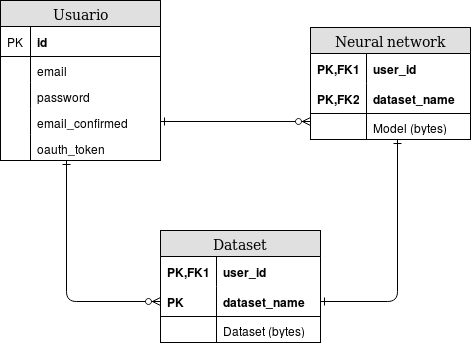
\includegraphics[width=0.8\textwidth]{er.png}
	\caption{Diagrama entidad relacción}\label{fig:er.png}
\end{figure}


Dentro de esta configuración tentemos que tener en cuenta que sólo el modelo del usuario esta dentro de la base de datos de manera que el resto se controla por software y se guarda dentro de los volúmenes de \emph{docker}


\subsection{Paso de datos}

El paso de datos entre los servicios se hace a través de SSH, esto se hace ya que nos proporciona seguridad. Otra opción es tener micro servidores de flask para exponer una \emph{API Rest} que nos permita hacer las operaciones de una forma más elegante. Esto dificulta algo la configuración interna poniendo más peso en el equipo de \emph{devops} pero nos permite tener un sistema mucho más desacoplado lo cual facilita el mantenimiento de ambas partes por separado.


\section{Diseño arquitectónico}
El diseño arquitectónico de la aplicación es uno muy parecido los que se usan en muchas páginas web para permitir mayor escalabilidad y picos de servicio sin caída del mismo. Simplemente se basa en permitir ejecutar múltiples instancias de los mismos objetos. Se podría ampliar la escalabilidad mediante \emph{reverse proxies} en distintos puntos de la arquitectura y con un servicio de caché como \href{https://redis.io/}{\emph{Redis}} antes de las bases de datos para permitir mayor velocidad de acceso. Si quisiésemos replicar micro servicios deberíamos poner un \emph{reverse proxy} o unirlos desde el que ya está.


\begin{figure}
	\centering
	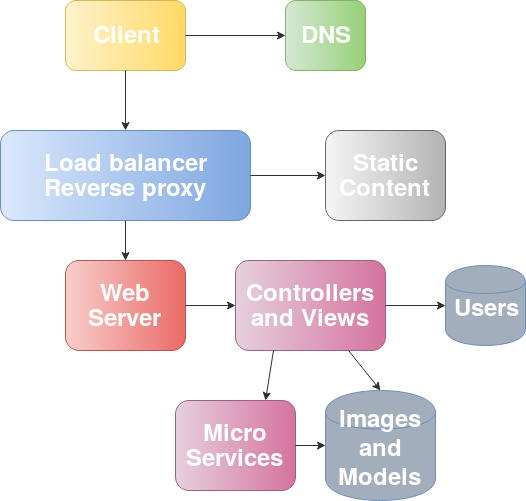
\includegraphics[width=0.8\textwidth]{Arquitecture.png}
	\caption{Arquitectura de la aplicación}\label{fig:Arquitecture.png}
\end{figure}

\subsection{Model View Controller (MVC)}

La parte de la aplicación tiene algo más de diseño en su interior. Para facilitar el desarrollo de futuros desarrolladores se ha decidido seguir la arquitectura ampliamente conocida como Modelo Vista Controlador o MVC. 

De esta manera logramos separar la vista con la cual interaccionará el usuario, con la lógica de interacción con la aplicación y del modelo de nuestro negocio. Gracias a esta abstracción podemos ocultar toda la complejidad de cada capa a los desarrolladores de las otras dos en caso de que nuestro negocio crezca hasta ese punto.

En nuestra estructura de archivos las vistas están bajo WhatAClass/WhatAClass/templates, los controladores se encuentran en WhatAClass/WhatAClass/blueprints y el único modelo explícito es el de usuario, situado en WhatAClass/WhatAClass/models, el resto son estructuras lógicas sobre el sistema de archivos.


\begin{figure}
	\centering
	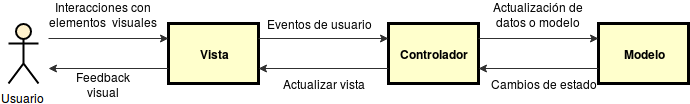
\includegraphics[width=0.8\textwidth]{mvc.png}
	\caption{Model view controller}\label{fig:mvc.png}
\end{figure}



\subsection{Factory Method}

En la aplicación que hemos creado se ha usado un factory method para permitir la creación de varias instancias de la aplicación de manera que se pueda escalar verticalmente (añadiendo más recursos en la misma máquina).

Esto también facilita la creación de la aplicación para programadores nuevos que desconozcan nuestro proyecto. Esto se debe a que las partes del factory method están bien establecidas y un programador que no conozca toda la aplicación puede solo añadir un par de líneas en el método que corresponda.


\section{Diseño procedimental}
En este apartado se expondrá que flujo sigue la información de forma general cuando se usa la aplicación.


\begin{figure}
	\centering
	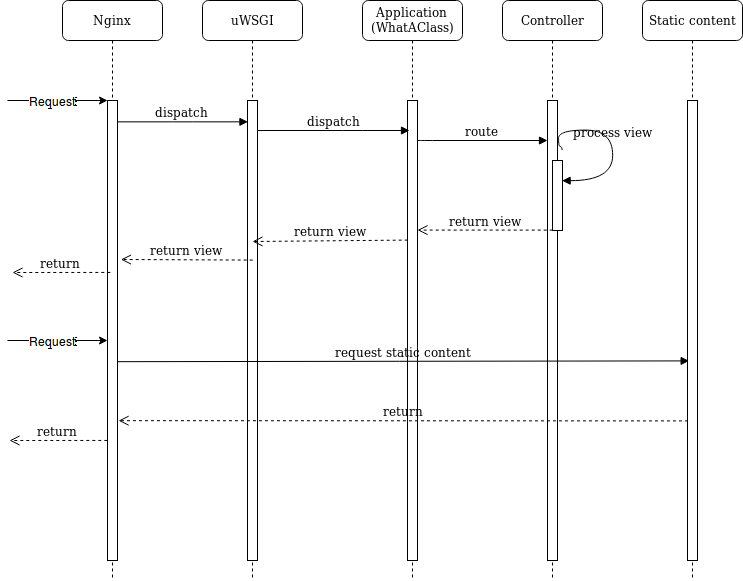
\includegraphics[width=0.8\textwidth]{Seq.png}
	\caption{Diagrama de secuencia}\label{fig:Seq.png}
\end{figure}

Como se puede observar la secuencia pasa por nginx para poder servir archivos estáticos a gran velocidad y para poder si se quisiese balancear la carga entre varios servidores de aplicación (uWSGI).


\section{Diseño de paquetes}


Programación a traves de metaclases (blueprints)


\subsection{Aplicación}
La aplicación esta descompuesta en el factory method (``app.py''), extensiones, formularios, modelo, utilidades y controladores.

Los controladores están en la carpeta blueprints pero se incluyen dentro de ``controllers.py'' para reducir el acoplamiento con el factory method.

Las utilidades tienen una configuración parecida a los controladores, las utilidades están el ``utils'' y se importan con ``util.py''.


\subsection{Configuración}
La configuración en general se implementa en la carpeta ``config'', de momento solo se dispone de una configuración (default) esto se debe a que gracias al uso de \emph{docker} y \emph{docker compose} podemos cambiar la configuración mediante las variables de entorno que estos pueden modificar, esto simplifica las configuraciones situacionales, ya que de esta manera toda la configuración que debamos cambiar podemos cambiarla en el archivo ``docker-compose.yml''.

\subsection{Tensorflow}
En el microservicio de tensorflow no necesitamos una estructura compleja ya que la biblioteca es suficientemente completa como para poder usarla con scripts sencillos.



